
% v2-acmsmall-sample.tex, dated March 6 2012
% This is a sample file for ACM small trim journals
%
% Compilation using 'acmsmall.cls' - version 1.3 (March 2012), Aptara Inc.
% (c) 2010 Association for Computing Machinery (ACM)
%
% Questions/Suggestions/Feedback should be addressed to => "acmtexsupport@aptaracorp.com".
% Users can also go through the FAQs available on the journal's submission webpage.
%
% Steps to compile: latex, bibtex, latex latex
%
% For tracking purposes => this is v1.3 - March 2012
\documentclass[prodmode,acmtecs]{acmsmall} % Aptara syntax
\usepackage[spanish,polish]{babel}
\usepackage[T1]{fontenc}
\usepackage{fancyvrb}
\usepackage{graphicx,hyperref}
\newcommand\cutout[1]{}


\usepackage[table]{xcolor}
\usepackage[utf8]{inputenc}
\usepackage[parfill]{parskip}
\usepackage{tabulary}
\PassOptionsToPackage{hyphens}{url}
\usepackage{hyperref}    
\usepackage[capitalize]{cleveref}


% Metadata Information
% !!! TODO: SET THESE VALUES !!!
\acmVolume{0}
\acmNumber{0}
\acmArticle{CFP}
\acmYear{0}
\acmMonth{0}

\newcounter{colstart}
\setcounter{page}{4}

\RecustomVerbatimCommand{\VerbatimInput}{VerbatimInput}%
{
%fontsize=\footnotesize,
fontfamily=\rmdefault
}


\newcommand{\UnderscoreCommands}{%\do\verbatiminput%
\do\citeNP \do\citeA \do\citeANP \do\citeN \do\shortcite%
\do\shortciteNP \do\shortciteA \do\shortciteANP \do\shortciteN%
\do\citeyear \do\citeyearNP%
}

\usepackage[strings]{underscore}



% Document starts
\begin{document}


\setcounter{colstart}{\thepage}

\acmArticle{CFP}
\title{\huge\sc SIGLOG Monthly 217}
\author{DAVID PURSER\affil{Max Planck Institute for Software Systems, Saarbr\"ucken}
\vspace*{-2.6cm}\begin{flushright}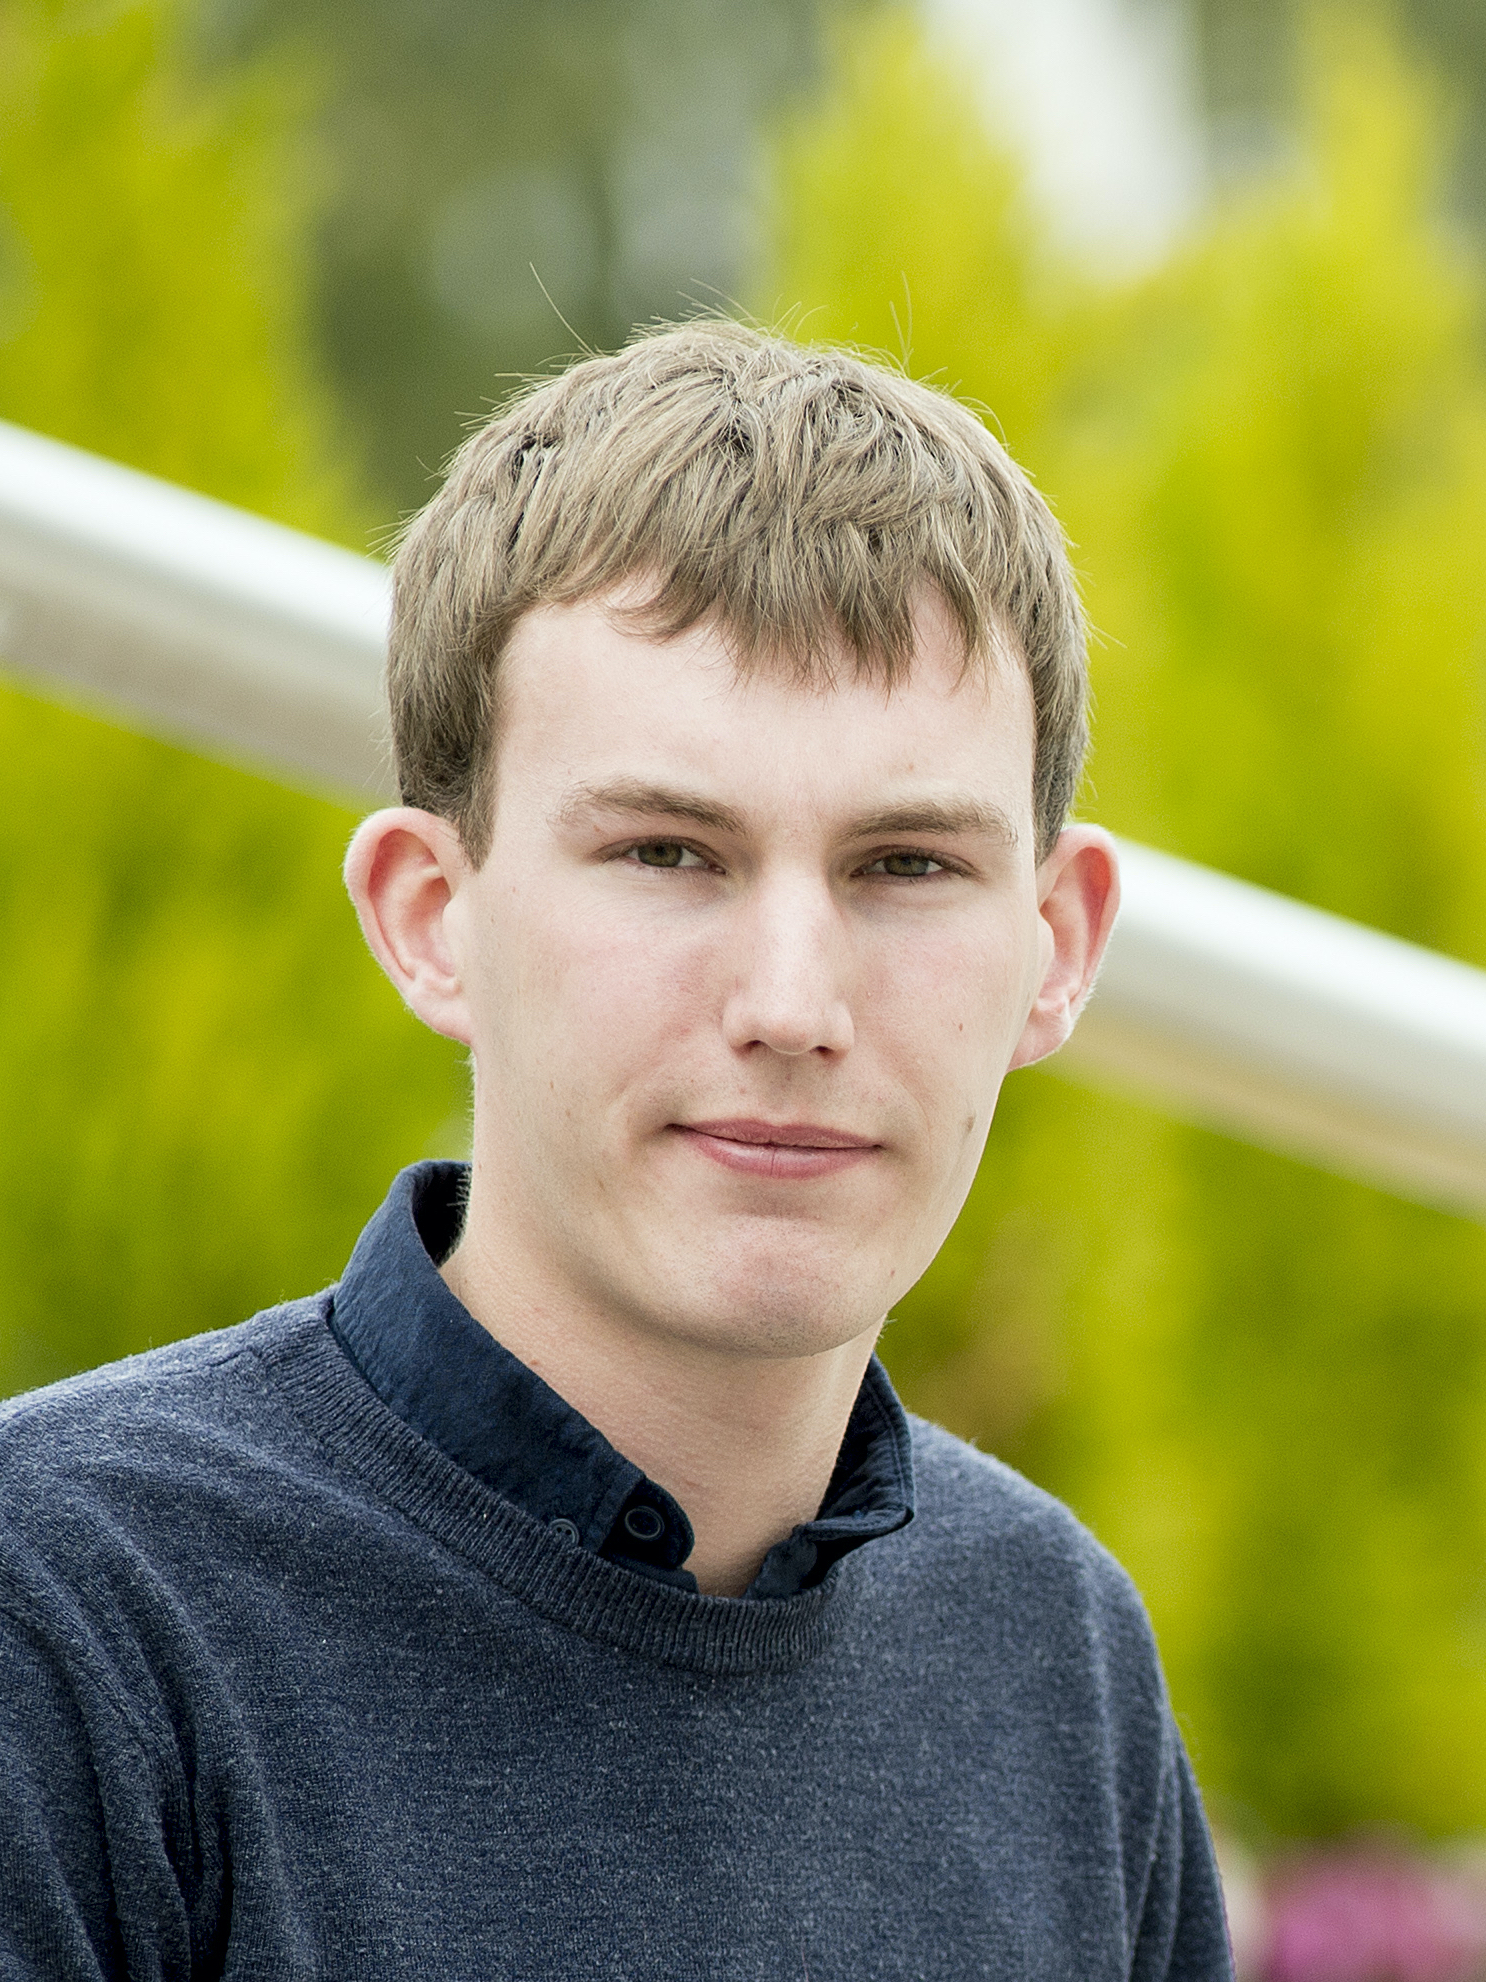
\includegraphics[width=30mm]{dp}\end{flushright}
}

\maketitlee

\href{https://lics.siglog.org/newsletters/}{Past Issues}
 - 
\href{https://lics.siglog.org/newsletters/inst.html}{How to submit an announcement}
\section{Table of Content}\begin{itemize}\item DEADLINES (\cref{deadlines}) 
 
\item CALLS 
 
\begin{itemize}\item HSCC 2022 (CALL FOR PAPERS) (\cref{HSCC2022})
\end{itemize} 
\item JOB ANNOUNCEMENTS 
 
\begin{itemize}\item Positions in the Formal Methods for Software Reliability group of TU Munich led by Prof. Jan Kretinsky (\cref{PositionsintheFormalMethodsforSoftwareReliabilitygroupofTUMunichledbyProfJanKretinsky})
\item PhD position in Formal Methods for Security and Concurrency at NTNU (\cref{PhDpositioninFormalMethodsforSecurityandConcurrencyatNTNU})
\end{itemize} 
\end{itemize}\section{Deadlines}\label{deadlines}\rowcolors{1}{white}{gray!25}\begin{tabulary}{\linewidth}{LL}Tenure track lecturer (Vrije Universiteit Brussel):  & Sept 6, 2021 (application deadline) \\
Applications for positions in Formal Methods for Software Reliability group (TU Munich):  & Sept 13, 2021 \\
CPP 2022:  & Sep 16, 2021 (Abstract submission deadline), Sep 22, 2021 (Paper submission deadline) \\
FLoC 2022:  & Sep 27, 2021 (Submission of workshop proposals deadline) \\
PhD position in Formal Methods for Security and Concurrency at NTNU:  & Sep 30, 2021 (Deadline) \\
HSCC 2022:  & Oct 29, 2021 (Submission deadline) \\
\end{tabulary}
\section{HSCC 2022: 25th ACM International Conference on Hybrid Systems Computation and Control }\label{HSCC2022}  Part of CPS-IoT Week 2022\\ 
  May 4-6, 2022, Milan, Italy\\ 
  \href{https://hscc.acm.org/2022/}{https://hscc.acm.org/2022/}\\ 
CALL FOR PAPERS 

\begin{itemize}\item  Hybrid Systems: Computation and Control (HSCC) 2022 is the 25th in a series of conferences focusing on original research on concepts, tools, and techniques from computer science, control theory, and applied mathematics for the analysis and control of hybrid dynamical systems, with an emphasis on computational aspects. By drawing on strategies from computation and control, the hybrid systems field offers techniques that are applicable to both man-made cyber-physical systems (ranging from small robots to global infrastructure networks) and natural systems (ranging from biochemical networks to physiological models). Papers in the conference are expected to range over a wide spectrum of topics from theoretical results to practical considerations, and from academic research to industrial adoption. 
 
\item  TOPICS 
 
  Topics of interest include, but are not limited to: 
 
\begin{itemize}\item  Mathematical foundations, computability and complexity
\item  Analysis, verification, validation, and testing
\item  Modeling paradigms and techniques
\item  Design, synthesis, planning, and control
\item  Programming and specification languages
\item  Network science and network-based control
\item  Security, privacy, and resilience for cyber-physical systems with focus on computation and control
\item  Safe autonomy, Artificial intelligence and Machine learning in CPS
\item  Software tools for the above topics
\item  Applications and industrial case studies in: automotive, transportation, autonomous systems, avionics, energy and power, robotics, medical devices, manufacturing, systems and synthetic biology, models for the life sciences, and other related areas.
\end{itemize} 
\item  SUBMISSION 
 
  HSCC invites submissions in two categories: (1) regular papers and (2) tool and case study papers. Submissions in both of these categories can be either long (10 pages max, 9pt font, two-column ACM format) or short papers (6 pages max, 9pt font, two-column ACM format). We will employ a double-blind reviewing process and will have a rebuttal phase to provide authors with the opportunity to reply to the reviewers’ concerns.  \href{https://easychair.org/conferences/?conf=hscc2022}{https://easychair.org/conferences/?conf=hscc2022} 
 
\item  IMPORTANT DATES (AOE) 
 
\rowcolors{1}{white}{gray!25}\begin{tabulary}{\linewidth}{LL}Submission deadline:  & Oct 29, 2021 \\
Tool/case study paper repeatability package submission deadline:  & Nov 01, 2021 \\
Rebuttal phase:  & December 15-17, 2021 \\
Acceptance/rejection notifications:  & Jan 17, 2022 \\
Posters/demos submission deadline:  & Jan 31, 2021 \\
\end{tabulary}
 
\end{itemize}\section{Positions in the Formal Methods for Software Reliability group of TU Munich led by Prof. Jan Kretinsky: }\label{PositionsintheFormalMethodsforSoftwareReliabilitygroupofTUMunichledbyProfJanKretinsky}  \href{https://www7.in.tum.de/~kretinsk/positions.html}{https://www7.in.tum.de/~kretinsk/positions.html}\\ 
JOB ANNOUNCEMENT 

\begin{itemize}\item  JOBS 
 
  We are looking for highly motivated candidates who will fit our enthusiastic and collaborative group spirit: 
 
\begin{itemize}\item  postdoc in the area of quantitative verification
\item  PhD students in quantitative verification and verified AI, possibly interested in co-developing Automata Tutor
\item  main developer of Automata Tutor 
\end{itemize} 
\item  TOPICS:  
 
\begin{itemize}\item  QUANTITATIVE VERIFICATION: analysis of probabilistic systems (Markov decision processes, stochastic games, chemical reaction networks), automata theory and temporal logic, machine learning in verification and verification of machine-learnt systems such as neural networks (also in industrial cooperation with AUDI), building model checkers (also verified by automated theorem proving) etc.
\item  AUTOMATA TUTOR (available at \href{https://automata-tutor.model.in.tum.de/}{https://automata-tutor.model.in.tum.de/}, described in publication \href{https://doi.org/10.1007/978-3-030-53291-8_1}{https://doi.org/10.1007/978-3-030-53291-8\_1}) is a tool to teach undergraduate students the basics of theoretical computer science. It offers automatic grading and feedback of various types of exercises. The tool has been used at dozens of universities around the world (including 5 times at TUM) and graded almost a million exercise solutions. 
\end{itemize} 
\item  Please see the full job posting for further information on the requirements, offer, conditions, salary and application process (deadline Sept 13, 2021). \href{https://www7.in.tum.de/~kretinsk/positions.html}{https://www7.in.tum.de/~kretinsk/positions.html} 
 
\item  Please contact jan.kretinsky@tum.de for any further information.  
 
\end{itemize}\section{PhD position in Formal Methods for Security and Concurrency at NTNU}\label{PhDpositioninFormalMethodsforSecurityandConcurrencyatNTNU}JOB ANNOUNCEMENT 

\begin{itemize}\item  We have a vacancy for a PhD researcher at the Systems Security Group in the Information Security Division of the Department of Information Security and Communication Technology at the Norwegian University of Science and Technology (NTNU) in the Gjøvik campus. 
 
\item  DEADLINE AND APPLICATION 
 
Deadline: Sep 30, 2021 
 
  Apply through the official announcement \href{https://www.jobbnorge.no/en/available-jobs/job/209665/phd-candidate-in-formal-methods-for-security-and-concurrency}{https://www.jobbnorge.no/en/available-jobs/job/209665/phd-candidate-in-formal-methods-for-security-and-concurrency}  
 
\item  TOPIC 
 
  The topic is generally placed at the intersection between security and concurrency with applications to many modern systems included under the term concurrency, such as distributed and communicating systems, multi-core or high-performance computing, or more generally systems of systems. The main focus of the topic will be on formal methods and tools applied to novel problems stemming from the combinations of security and highly complex concurrent systems. Depending on the inclinations and skills of the applicant, the work can include theoretical investigations as well as development and improvement of existing methods and tools for solving verification challenges in such modern applications; but the work can also include modelling and verification of real-world protocols pertaining to, e.g., IoT, Smart Grids, or Smart Contracts. Therefore, the research tasks can be anything from more theoretical, designing new formalisms and algorithms, to more practical, implementing modules, extensions, or new tools. If the work will go in a more theoretical direction, the candidate can expect to look into formalisms such as process algebras and their methods such as bisimulations, or into concurrency models and the challenges these bring to security, or into more mathematical topics including logics, relational algebras, automata, etc. If the work will go in a more practical direction, the candidate can expect to work with security verification tools such as Isabelle or Tamarin. 
 
\item  Contact: christian.johansen@ntnu.no  (for inquires about the position)  
 
\item  For further details regarding application process, selection criteria, salary, conditions and further information please see the full advert: \href{https://www.jobbnorge.no/en/available-jobs/job/209665/}{https://www.jobbnorge.no/en/available-jobs/job/209665/} 
 
\end{itemize}


To the \href{http://siglog.org/}{SIGLOG} or \href{https://lics.siglog.org}{LICS} website\end{document}